%============================================================================%
%
%	DOCUMENT DEFINITION
%
%============================================================================%

%we use article class because we want to fully customize the page and don't use a cv template
\documentclass[10pt,A4]{article}	


%----------------------------------------------------------------------------------------
%	ENCODING
%----------------------------------------------------------------------------------------

% we use utf8 since we want to build from any machine
\usepackage[utf8]{inputenc}		

%----------------------------------------------------------------------------------------
%	LOGIC
%----------------------------------------------------------------------------------------

% provides \isempty test
\usepackage{xstring, xifthen}

%----------------------------------------------------------------------------------------
%	FONT BASICS
%----------------------------------------------------------------------------------------

% some tex-live fonts - choose your own

%\usepackage[defaultsans]{droidsans}
%\usepackage[default]{comfortaa}
%\usepackage{cmbright}
\usepackage[default]{raleway}
%\usepackage{fetamont}
%\usepackage[default]{gillius}
%\usepackage[light,math]{iwona}
%\usepackage[thin]{roboto} 

% set font default
\renewcommand*\familydefault{\sfdefault} 	
\usepackage[T1]{fontenc}

% more font size definitions
\usepackage{moresize}

%----------------------------------------------------------------------------------------
%	FONT AWESOME ICONS
%---------------------------------------------------------------------------------------- 

% include the fontawesome icon set
\usepackage{fontawesome}

% use to vertically center content
% credits to: http://tex.stackexchange.com/questions/7219/how-to-vertically-center-two-images-next-to-each-other
\newcommand{\vcenteredinclude}[1]{\begingroup
\setbox0=\hbox{\includegraphics{#1}}%
\parbox{\wd0}{\box0}\endgroup}

% use to vertically center content
% credits to: http://tex.stackexchange.com/questions/7219/how-to-vertically-center-two-images-next-to-each-other
\newcommand*{\vcenteredhbox}[1]{\begingroup
\setbox0=\hbox{#1}\parbox{\wd0}{\box0}\endgroup}

% icon shortcut
\newcommand{\icon}[3] { 							
	\makebox(#2, #2){\textcolor{maincol}{\csname fa#1\endcsname}}
}	

% icon with text shortcut
\newcommand{\icontext}[4]{ 						
	\vcenteredhbox{\icon{#1}{#2}{#3}}  \hspace{2pt}  \parbox{0.9\mpwidth}{\textcolor{#4}{#3}}
}

% icon with website url
\newcommand{\iconhref}[5]{ 						
    \vcenteredhbox{\icon{#1}{#2}{#5}}  \hspace{2pt} \href{#4}{\textcolor{#5}{#3}}
}

% icon with email link
\newcommand{\iconemail}[5]{ 						
    \vcenteredhbox{\icon{#1}{#2}{#5}}  \hspace{2pt} \href{mailto:#4}{\textcolor{#5}{#3}}
}

%----------------------------------------------------------------------------------------
%	PAGE LAYOUT  DEFINITIONS
%----------------------------------------------------------------------------------------

% page outer frames (debug-only)
% \usepackage{showframe}		

% we use paracol to display breakable two columns
\usepackage{paracol}

% define page styles using geometry
\usepackage[a4paper]{geometry}

% remove all possible margins
\geometry{top=1cm, bottom=1cm, left=1cm, right=1cm}

\usepackage{fancyhdr}
\pagestyle{empty}

% space between header and content
% \setlength{\headheight}{0pt}

% indentation is zero
\setlength{\parindent}{0mm}

%----------------------------------------------------------------------------------------
%	TABLE /ARRAY DEFINITIONS
%---------------------------------------------------------------------------------------- 

% extended aligning of tabular cells
\usepackage{array}

% custom column right-align with fixed width
% use like p{size} but via x{size}
\newcolumntype{x}[1]{%
>{\raggedleft\hspace{0pt}}p{#1}}%


%----------------------------------------------------------------------------------------
%	GRAPHICS DEFINITIONS
%---------------------------------------------------------------------------------------- 

%for header image
\usepackage{graphicx}

% use this for floating figures
% \usepackage{wrapfig}
% \usepackage{float}
% \floatstyle{boxed} 
% \restylefloat{figure}

%for drawing graphics		
\usepackage{tikz}				
\usetikzlibrary{shapes, backgrounds,mindmap, trees}

%----------------------------------------------------------------------------------------
%	Color DEFINITIONS
%---------------------------------------------------------------------------------------- 
\usepackage{transparent}
\usepackage{color}

% primary color
\definecolor{maincol}{RGB}{ 225, 0, 0 }

% accent color, secondary
% \definecolor{accentcol}{RGB}{ 250, 150, 10 }

% dark color
\definecolor{darkcol}{RGB}{ 70, 70, 70 }

% light color
\definecolor{lightcol}{RGB}{245,245,245}


% Package for links, must be the last package used
\usepackage[hidelinks]{hyperref}

% returns minipage width minus two times \fboxsep
% to keep padding included in width calculations
% can also be used for other boxes / environments
\newcommand{\mpwidth}{\linewidth-\fboxsep-\fboxsep}
	


%============================================================================%
%
%	CV COMMANDS
%
%============================================================================%

%----------------------------------------------------------------------------------------
%	 CV LIST
%----------------------------------------------------------------------------------------

% renders a standard latex list but abstracts away the environment definition (begin/end)
\newcommand{\cvlist}[1] {
	\begin{itemize}{#1}\end{itemize}
}

%----------------------------------------------------------------------------------------
%	 CV TEXT
%----------------------------------------------------------------------------------------

% base class to wrap any text based stuff here. Renders like a paragraph.
% Allows complex commands to be passed, too.
% param 1: *any
\newcommand{\cvtext}[1] {
	\begin{tabular*}{1\mpwidth}{p{0.98\mpwidth}}
		\parbox{1\mpwidth}{#1}
	\end{tabular*}
}

%----------------------------------------------------------------------------------------
%	CV SECTION
%----------------------------------------------------------------------------------------

% Renders a a CV section headline with a nice underline in main color.
% param 1: section title
\newcommand{\cvsection}[1] {
	\vspace{14pt}
	\cvtext{
		\textbf{\LARGE{\textcolor{darkcol}{\uppercase{#1}}}}\\[-4pt]
		\textcolor{maincol}{ \rule{0.1\textwidth}{2pt} } \\
	}
}

%----------------------------------------------------------------------------------------
%	META SKILL
%----------------------------------------------------------------------------------------

% Renders a progress-bar to indicate a certain skill in percent.
% param 1: name of the skill / tech / etc.
% param 2: level (for example in years)
% param 3: percent, values range from 0 to 1
\newcommand{\cvskill}[3] {
	\begin{tabular*}{1\mpwidth}{p{0.72\mpwidth}  r}
 		\textcolor{black}{\textbf{#1}} & \textcolor{maincol}{#2}\\
	\end{tabular*}%
	
	\hspace{4pt}
	\begin{tikzpicture}[scale=1,rounded corners=2pt,very thin]
		\fill [lightcol] (0,0) rectangle (1\mpwidth, 0.15);
		\fill [maincol] (0,0) rectangle (#3\mpwidth, 0.15);
  	\end{tikzpicture}%
}


%----------------------------------------------------------------------------------------
%	 CV EVENT
%----------------------------------------------------------------------------------------

% Renders a table and a paragraph (cvtext) wrapped in a parbox (to ensure minimum content
% is glued together when a pagebreak appears).
% Additional Information can be passed in text or list form (or other environments).
% the work you did
% param 1: time-frame i.e. Sep 14 - Jan 15 etc.
% param 2:	 event name (job position etc.)
% param 3: Customer, Employer, Industry
% param 4: Short description
% param 5: work done (optional)
% param 6: technologies include (optional)
% param 7: achievements (optional)
\newcommand{\cvevent}[7] {
	
	% we wrap this part in a parbox, so title and description are not separated on a pagebreak
	% if you need more control on page breaks, remove the parbox
	\parbox{\mpwidth}{
		\begin{tabular*}{1\mpwidth}{p{0.72\mpwidth}  r}
	 		\textcolor{black}{\textbf{#2}} & \colorbox{maincol}{\makebox[0.25\mpwidth]{\textcolor{white}{#1}}} \\
			\textcolor{maincol}{\textbf{#3}} & \\
		\end{tabular*}\\[8pt]
	
		\ifthenelse{\isempty{#4}}{}{
			\cvtext{#4}\\
		}
	}

	\ifthenelse{\isempty{#5}}{}{
		\vspace{9pt}
		{#5}
	}

	\ifthenelse{\isempty{#6}}{}{
		\vspace{9pt}
		\cvtext{\textbf{Technologies include:}}\\
		{#6}
	}

	\ifthenelse{\isempty{#7}}{}{
		\vspace{9pt}
		\cvtext{\textbf{Achievements include:}}\\
		{#7}
	}
	\vspace{14pt}
}

%----------------------------------------------------------------------------------------
%	 CV META EVENT
%----------------------------------------------------------------------------------------

% Renders a CV event on the sidebar
% param 1: title
% param 2: subtitle (optional)
% param 3: customer, employer, etc,. (optional)
% param 4: info text (optional)
\newcommand{\cvmetaevent}[4] {
	\textcolor{maincol} {\cvtext{\textbf{\begin{flushleft}#1\end{flushleft}}}}

	\ifthenelse{\isempty{#2}}{}{
	\textcolor{darkcol} {\cvtext{\textbf{#2}} }
	}

	\ifthenelse{\isempty{#3}}{}{
		\cvtext{{ \textcolor{darkcol} {#3} }}\\
	}

	\cvtext{#4}\\[14pt]
}

%---------------------------------------------------------------------------------------
%	QR CODE
%----------------------------------------------------------------------------------------

% Renders a qrcode image (centered, relative to the parentwidth)
% param 1: percent width, from 0 to 1
\newcommand{\cvqrcode}[1] {
	\begin{center}
		
\includegraphics[width={#1}\mpwidth]{qrcode}
	\end{center}
}


%============================================================================%
%
%
%
%	DOCUMENT CONTENT
%
%
%
%============================================================================%
\begin{document}
\columnratio{0.31}
\setlength{\columnsep}{2.2em}
\setlength{\columnseprule}{4pt}
\colseprulecolor{lightcol}
\begin{paracol}{2}
\begin{leftcolumn}
%---------------------------------------------------------------------------------------
%	META IMAGE
%----------------------------------------------------------------------------------------
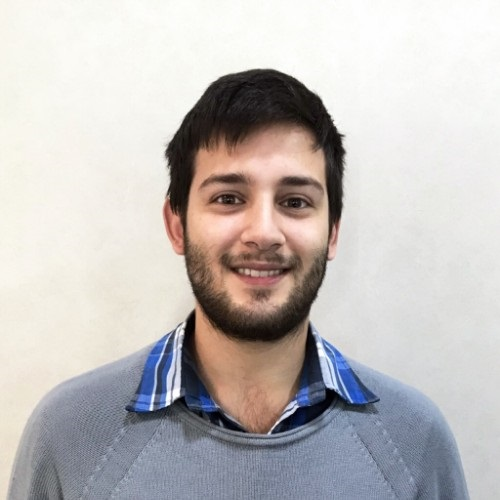
\includegraphics[width=\linewidth]{untitled.jpg}	%trimming relative to image size

%---------------------------------------------------------------------------------------
%	META SKILLS
%----------------------------------------------------------------------------------------
\cvsection{HABILIDADES}

\cvskill{Python} {2+ yrs} {1} \\[-2pt]

\cvskill{SQL} {2+ yrs} {1} \\[-2pt]

\cvskill{Machine Learning} {2+ yrs} {1} \\[-2pt]

\cvskill{Deep Learning} {2+ yrs} {0.75} \\[-2pt]

\cvskill{Alteryx} {2+ yrs} {0.75} \\[-2pt]

\cvskill{GIT} {1+ yrs} {0.75} \\[-2pt]

\cvskill{PowerBI} {1+ yrs} {0.75} \\[-2pt]

\cvskill{Ui Path} {1+ yrs} {0.5} \\[-2pt]

\cvskill{R} {1+ yrs} {0.5} \\[-2pt]


\vfill\null
\cvsection{CONTACTO}
	
\icontext{MapMarker}{12}{Sarmiento 1720 10A\\Rosario, Santa Fe}{black}\\[6pt]
\icontext{MobilePhone}{12}{+54 3416751379}{black}\\[6pt]
\iconemail{Envelope}{12}{estebancometto@gmail.com}{estebancometto@gmail.com}{black}\\[6pt]

\vfill\null
\cvqrcode{0.7}

%---------------------------------------------------------------------------------------
%	EDUCATION
%----------------------------------------------------------------------------------------
\newpage
\cvsection{EDUCACIÓN}

\cvmetaevent
{2013 - 2017}
{Licenciatura en Estadística}
{Universidad Nacional de Rosario}
{Cursado terminado en 2017, en este momento adeudando tesina}
% {Main thematic priority of those master studies was numerical time series analysis of non-linear dynamical systems.
% Besides data analysis and transformation, great importance was attached to fast algorithms and efficient software
% architecture.

% In the master thesis a numerical approach for the detection of the direction of interaction was proposed. Analysis of
% this new approach was performed with the help computer simulations to find out its limits and to compare it to another
% commonly used approaches.

% This numerical approach was highly optimised for cluster computing and implemented in c++ . For those purposes a
% distributed computing cluster had to be set up and administrated.}

\cvmetaevent
{2008 - 2012}
{Bachiller en Economía}
{Escuela de Enseñanza Media Dr. Luis Maria Drago}
% {The topic for the bachelor's thesis was 'Feshbach resonance'. A numerical application was built to calculate the diagrams.}

\vfill\null
\cvqrcode{0.7}

%---------------------------------------------------------------------------------------
%	CERTIFICATION
%----------------------------------------------------------------------------------------
\newpage
\cvsection{CERTIFICACIONES}

\cvmetaevent
{Data Scientist with Python Track}
{DataCamp}
{15 de Mayo de 2020}
{100 horas de cursado sobre técnicas estadísticas y de aprendizaje automático con programación Python para analizar e
interpretar datos complejos.}

\cvmetaevent
{Machine Learning A-Z: Hands-On Python and R in Data Science}
{Udemy}
{5 de Agosto de 2020}
{15 horas de cursado sobre grandes ideas en el aprendizaje automático, como cómo construir y evaluar modelos predictivos.}


\vfill
\cvqrcode{0.7}

\newpage
\mbox{} % hotfix to place qrcode on the bottom when there are not other elements
\vfill
\cvqrcode{0.7}

\end{leftcolumn}
\begin{rightcolumn}
%---------------------------------------------------------------------------------------
%	TITLE  HEADER
%----------------------------------------------------------------------------------------
\fcolorbox{white}{darkcol}{\begin{minipage}[c][3.5cm][c]{1\mpwidth}
	\begin {center}
		\HUGE{ \textbf{ \textcolor{white}{ \uppercase{ ESTEBAN COMETTO } } } } \\[-24pt]
		\textcolor{white}{ \rule{0.1\textwidth}{1.25pt} } \\[4pt]
		\large{ \textcolor{white} {Data Scientist and Python Developer} }
	\end {center}
\end{minipage}} \\[14pt]
\vspace{-12pt}

%---------------------------------------------------------------------------------------
%	PROFILE
%----------------------------------------------------------------------------------------
\vfill\null
\cvsection{PERFIL}

\cvtext{Data Scientist con fuertes habilidades teóricas y apasionado del análisis de datos.\\

Python Developer, especializado en machine learning y automatización de procesos y con conocimientos de ciertas áreas como
web scraping y web browser automation.\\

Método de trabajo estructurado y orientado al cliente, centrado en la calidad y la mantenibilidad. Altamente motivado para
trabajar en equipo, tanto cómodo en grandes empresas como en pequeños equipos. \\

}

%---------------------------------------------------------------------------------------
%	WORK EXPERIENCE
%----------------------------------------------------------------------------------------
\vfill\null
\cvsection{EXPERIENCIA LABORAL}

\cvevent
	{Sep 15 - NOW}
	{DevOps/FullStack developer}
	{Research and Development}
	{A large IAM project required an intuitive interface for role-based access and rights management. At the same time, new workfows for role based access, life time and monitoring had to be established}
	{\cvlist{
		\item Creation of a web portal for role- and rights management
		\item Establishing a connection to the existing MicroFocus role solution
		\item Development of new role-based workfows and processes, as well as training and support
		\item Maintenance of existing infrastructure
	}}
	{\cvlist {
		\item Django for the roles- and rights management tool backend (backend is a REST interface)
		\item Angular for the easy frontend interaction
		\item HTML5/CSS3/Bootstrap3 for the frontend
		\item Ansible + Docker for 1-click deployments
	}}
	{\cvlist{
		\item A web based tool for an intuitive role assignment and administration
		\item Online overview of company structures, projects, etc
		\item Tools for role review, reporting and troubleshooting
	}}

\vfill\null
\cvevent
	{Jan 15 - Sep 15}
	{DevOps engineer}
	{Research and Development}
	{Responsible for infrastructure architecture with regard on the future development and tool selection in the field of identity and access management}
	{\cvlist{
		\item Selection of future-proof tools for a large infrastructure
		\item Infrastructure migration into a cloudstack cloud
		\item Quality assurance in terms of documentation
		\item Tool development for infrastructure overview
		\item Development of Ansible modules for client
	}}
	{\cvlist {
		\item Python for custom tool development
		\item Ansible for infrastructure migration and cloud configuration
		\item SLES12
		\item Django for Visualization
	}}
	{\cvlist{
		\item Ansible module for SLES12 System + Package registration
		\item Python tool for ACL-administration in cloud
		\item Fully automated migration of old systems into cloud with Ansible playbooks/roles
		\item Django tool on LDAP - Schema Review
	}}

\vfill\null
\cvevent
	{Mar 14 - Jan 15}
	{Systems Analyst}
	{Research and Development}
	{Responsible for infrastructure architecture / automaton as well as custom tool development on a project for directory services and identity / access management in a large heterogeneous environment.}
	{\cvlist{
		\item Design and implementation of update and deployment process automaton
		\item Quality assurance by design of infrastructure monitoring, centralized logging solutions and documentation
		\item Customized tool creation for ldap operations
		\item Installation and maintenance of single sign on solutions
		\item Customer support in ldap / infrastructural / programming concerns
	}}
	{\cvlist {
		\item Ansible for infrastructure automaton and configuration management
		\item Python for custom Tool development
		\item nxLog + rsyslog + graylog for logging infrastructure
		\item NOVELL eDirectory
		\item Shibboleth as identity Provider combined with ldap
		\item SLES11
		\item Git for configuration and documentation versioning
	}}
	{\cvlist{
		\item Drastically accelerated (~20x faster) the update process and improved its reliability by introduction of centralized configuration management
		\item Extended the python-ldap library with interfaces for simplified access and modification of LDAP-Objects and searches
		\item  Introduction of a complete and reliable centralized logging solution including log filtering and alerting for both windows and Linux systems
	}}

\vfill\null
\cvevent
	{Sep 13 - Mar 14}
	{Systems Analyst}
	{Tourism industry}
	{Responsible for data transformation and tool customization on a migration (legacy c++ code from Solaris to Linux systems) project. The tasks include}
	{\cvlist{
		\item Tool development for identification of critical spots in code
		\item Legacy code analysis
		\item Quality assurance
		\item Department-wide training in python
		\item Consulting in topics of migration to Git
	}}
	{\cvlist {
		\item Python
		\item Git
		\item Linux (Debian)
	}}
	{\cvlist{
		\item Implementing code coverage and dynamic code checker for c++ legacy source code based on gcov
		\item Introduction of Python + Environment in project
	}}

\vfill\null
\cvevent
	{Oct 12 - Sep 13}
	{Systems Analyst}
	{Tourism industry}
	{Responsible for the infrastructure including performance and quality assurance on a large social media project.}
	{\cvlist{
		\item Organization and care of a cloud network (Debian systems)
		\item Support for software developers
		\item Configuration of open source tools for code quality and documentation
		\item Implementation of performance checks
		\item Implementation of automated reports on code quality and performance
	}}
	{\cvlist {
		\item Python + Django for tool development
		\item Sonar as static and dynamic tool for code analysis
		\item OpenLDAP for user rights management
		\item JIRA as the issue tracking/SCRUM tool
	}}
	{\cvlist{
		\item Customized wiki and documentation application for developers with Jenkins and Git integration
		\item Django web application to test the product performance using selenium tests in background with customizable tests / test
environments ad a graphical evaluation using the jqPlot library (also Jaiascript / jQuery)
		\item Improvement of the overall code quality by raising test coverage (+ \~30\%) and identification + elimination of potential code flaws
	}}

\vfill\null
\cvevent
	{Oct 11 - Oct 12}
	{IT Consultant}
	{Accenture Tech. Solutions}
	{Large public service project with the goal to establish a platform for handling of finance processes with a very high number of transactions. Main focus was the migration of legacy data, by assuring data quality and transformation into various formats}
	{\cvlist{
		\item Customer consulting with regard to loading / unloading interfaces
		\item Definition of requirements for transformation of legacy data
		\item Implementation of algorithms for data transformation
		\item Tool development for secure data transport
		\item Tool development for tests of data quality/interface implementation
	}}
	{\cvlist {
		\item Standard Linux tools, such as awk, sed, grep, ...
		\item Python for in-depth data analysis
		\item Java for transport layers
		\item IBM DataStage
	}}
	{\cvlist{
		\item Definition of uniform standards
		\item Introduction of the standard Linux stack as global toolset for data analysis in project
	}}

% hotfixes to create fake-space to ensure the whole height is used
\mbox{}
\vfill
\mbox{}
\vfill
\mbox{}
\vfill
\mbox{}
\end{rightcolumn}
\end{paracol}
\end{document}

